\documentclass[11pt,a4paper]{article}

\usepackage[margin=2.5cm]{geometry}
\usepackage[T1]{fontenc}
\usepackage{lmodern}
\usepackage{microtype}
\usepackage{booktabs}
\usepackage{longtable}
\usepackage{xcolor}
\usepackage{listings}
\usepackage{amsmath}
\usepackage{amssymb}
\usepackage{enumitem}
\usepackage{graphicx}
\usepackage{float}
\usepackage{tikz}
\usepackage[hidelinks]{hyperref}
\usepackage[capitalise]{cleveref}
\graphicspath{{figures/}{../resources/Icons/}}

\definecolor{codebg}{RGB}{247,247,247}
\definecolor{codekey}{RGB}{20,80,160}
\definecolor{codestr}{RGB}{150,60,20}
\definecolor{warnbg}{RGB}{255,248,235}
\definecolor{warnrule}{RGB}{200,140,40}

\lstdefinestyle{json}{
  basicstyle=\ttfamily\footnotesize,
  backgroundcolor=\color{codebg},
  breaklines=true, columns=fullflexible, keepspaces=true,
  showstringspaces=false, frame=single, framerule=0pt, framesep=6pt,
  xleftmargin=6pt, stringstyle=\color{codestr},
  literate=*{:}{{{\color{codekey}:}}}{1}{\{}{{{\color{codekey}\{}}}{1}{\}}{{{\color{codekey}\}}}}{1},
}
\lstdefinestyle{plain}{
  basicstyle=\ttfamily\footnotesize, backgroundcolor=\color{codebg},
  breaklines=true, columns=fullflexible, keepspaces=true,
  showstringspaces=false, frame=single, framerule=0pt, framesep=6pt, xleftmargin=6pt,
}
\lstset{style=json}

\newcommand{\code}[1]{\texttt{\small #1}}
\newcommand{\file}[1]{\texttt{\small #1}}
\let\oldus\_
\renewcommand{\_}{\oldus\allowbreak}   % long code names may break after an underscore

\newcommand{\ghbase}{https://github.com/ArashMassoudieh/OpenHydroQual/blob/master}
\newcommand{\ghtree}{https://github.com/ArashMassoudieh/OpenHydroQual/tree/master}
\newcommand{\exfile}[1]{\href{\ghbase/#1}{\file{#1}}}
\newcommand{\exdir}[1]{\href{\ghtree/#1}{\file{#1}}}

\newenvironment{caution}
  {\par\medskip\noindent
\begin{tikzpicture}\node[draw=warnrule,fill=warnbg,line width=0.8pt,
   rounded corners=2pt,inner sep=8pt,text width=\dimexpr\textwidth-20pt\relax,align=left]\bgroup}
  {\egroup;\end{tikzpicture}\par\medskip}

\title{\textbf{Hydrologic Response Units in OpenHydroQual}\\[0.3em]
       \large The HRU and Urban HRU composite blocks (and the legacy Mixed HRU)}
\author{}
\date{}

\begin{document}
\maketitle
\vspace{-2.5em}

\begin{abstract}
\noindent
A hydrologic response unit (HRU) in OpenHydroQual is a composite block that bundles the surface,
soil and groundwater stores of one piece of land and the connectors between them, so that a
sub-catchment is added to a model as a single object with a single set of properties. This document
describes the two HRUs offered in the interface: the \code{Hydrologic\_Response\_Unit} (``HRU''), a
single infiltrating surface over a three-layer soil column and a groundwater cell, and the
\code{Urban\_HRU}, which adds an impervious surface, internal routing reaches, a groundwater cell under
the whole unit recharged through the unsaturated conductivity of the bottom soil layer, unconfined
groundwater storage, layer-specific soil parameters and two calibration multipliers. It also
documents the \code{Mixed\_Hydrologic\_Response\_Unit}, the predecessor of the Urban HRU, which is no
longer listed in the interface but is kept so that existing models load, and shows with a pair of
example models run with identical inputs why it was replaced. For each unit the document sets out the
members and connectors, the equation of each flux, how the plan area is divided, how the vertical
geometry and the initial state follow from a few properties, and how the impervious fraction should
be estimated.
\end{abstract}

\tableofcontents

%==========================================================================================
\section{Which HRU to use}

\begin{table}[H]
\centering\small
\begin{tabular}{p{3.6cm}p{3.4cm}p{3.6cm}p{3.6cm}}
\toprule
 & \code{Hydrologic\_Response\_Unit} & \code{Mixed\_Hydrologic\_Response\_Unit} & \code{Urban\_HRU} \\
\midrule
File & \file{hydrologic\_response\_unit.json} & \file{mixed\_hydrologic\_response\_unit.json} & \file{urban\_hru.json} \\
Surfaces & one, infiltrating & pervious + impervious & pervious + impervious \\
Internal routing reaches & none & one per surface & one per surface \\
Soil parameters & one set & one set & one set per layer \\
Groundwater area & $A$ & $A(1-f_i)$ & $A$ (whole unit) \\
Recharge conductivity & constant \code{recharge\_K} & constant \code{recharge\_K} & $K_{sat,3}\,k_r(S_{e,3})$ \\
Groundwater storage & user $S_s$ & user $S_s$ & unconfined, $S_s=\phi/b$ \\
Calibration multipliers & --- & --- & \code{impervious\_multiplier}, \code{K\_sat\_scale} \\
In the template list & yes & no (legacy) & yes \\
Icon & 
\includegraphics[height=1.4cm]{hydrologic_response_unit.png} &
       
\includegraphics[height=1.4cm]{mixed_hydrologic_response_unit.png} &
       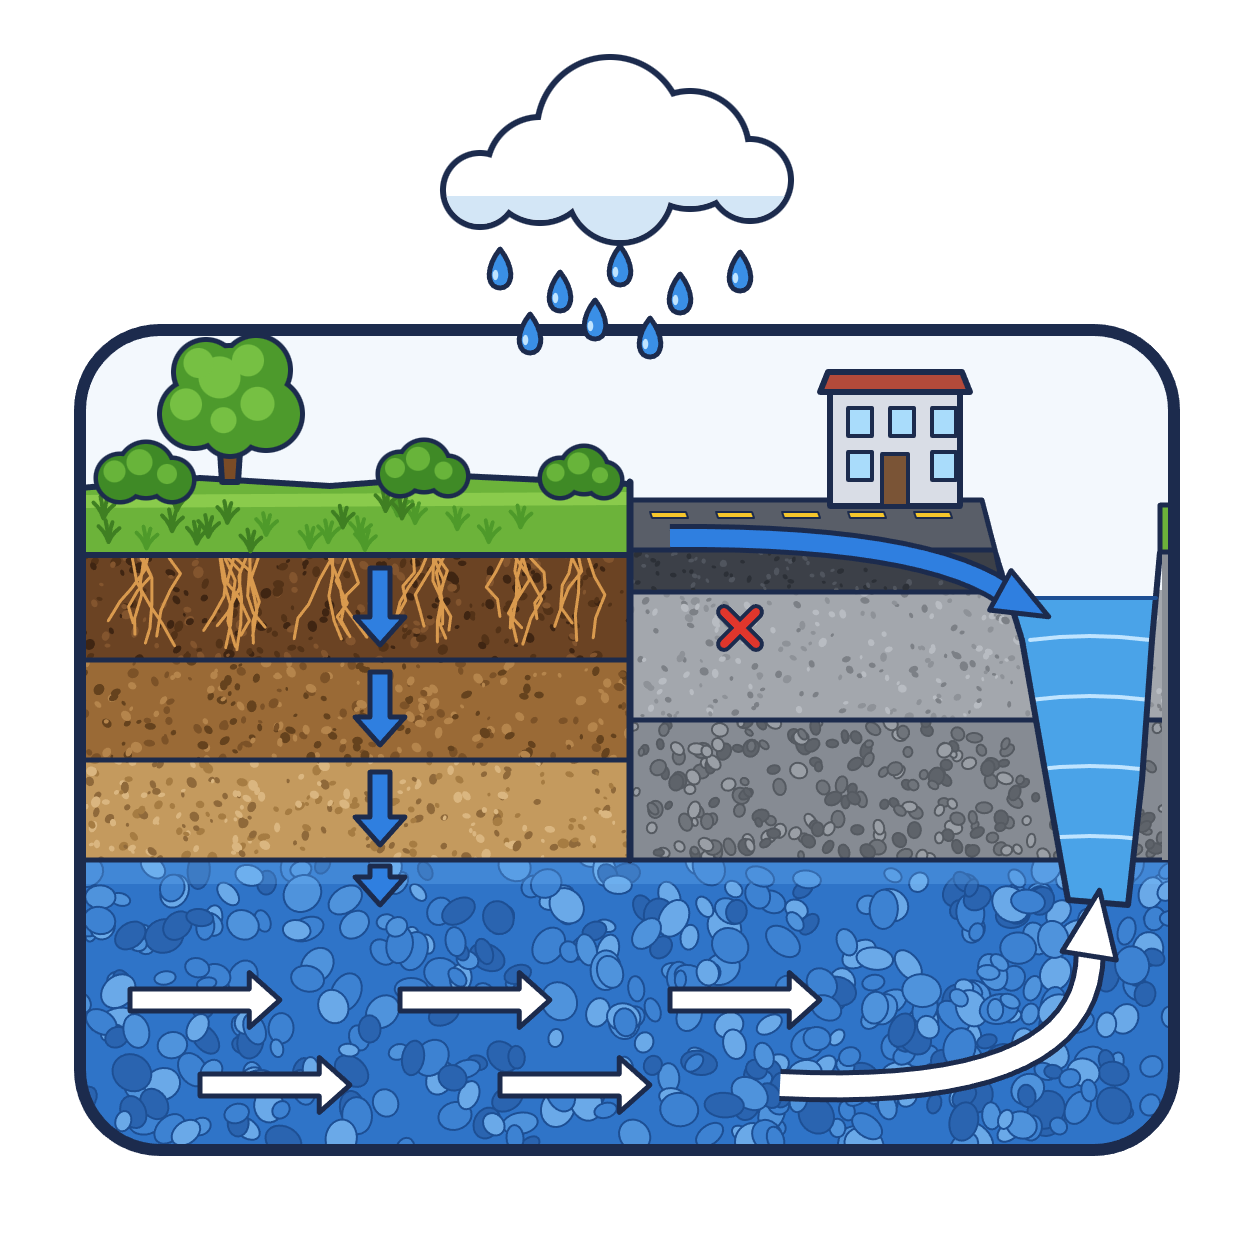
\includegraphics[height=1.4cm]{urban_hru.png} \\
\bottomrule
\end{tabular}
\caption{The three HRU composites. $A$ is the plan area, $f_i$ the impervious fraction, $\phi$ the
groundwater porosity and $b$ the groundwater thickness.}
\end{table}

Use the \textbf{HRU} for land without significant impervious cover --- forest, fields, parks,
hillslopes --- and for cascades of units where the overland flow of one unit runs onto the next
(\cref{sec:hru}). Use the \textbf{Urban HRU} wherever part of the land is impervious and drains
directly to a stream or storm drain: it partitions the area, routes each surface separately, and its
subsurface (\cref{sec:urbanspec}) stays physically sensible when the water table lies well below the
soil column. The \textbf{Mixed HRU} is superseded by the Urban HRU; it remains in
\file{resources/} so that existing models open, and because the Urban HRU loads its two outlet link
types from it (\cref{sec:mixedspec}).

%==========================================================================================
\section{Elements shared by all units}
\label{sec:shared}
All three units build their subsurface from the same members: three \code{Soil} layers and a
\code{Groundwater cell}, connected by infiltration, two percolation links and a recharge link. The
geometry and the soil-water relations below apply to all of them; the units differ in the plan areas
they give these members and in the recharge link (\cref{sec:hru,sec:mixedspec,sec:urbanspec}).

\subsection{Vertical geometry}
The user gives three levels; everything else is derived:

\begin{table}[H]
\centering\small
\begin{tabular}{lll}
\toprule
Member & Thickness & Bottom elevation \\
\midrule
\code{Catchment}, \code{Impervious\_Catchment}, reaches & --- & $z_s$ (\code{surface\_elevation}) \\
\code{Soil\_1} & $D/7$ & $z_s-D/7$ \\
\code{Soil\_2} & $2D/7$ & $z_s-3D/7$ \\
\code{Soil\_3} & $4D/7$ & $z_s-D$ \\
\code{Groundwater} & $b$ (\code{groundwater\_thickness}) & $z_s-D-b$ \\
\bottomrule
\end{tabular}
\end{table}

\noindent $D$ is \code{depth\_to\_groundwater}. The $1\!:\!2\!:\!4$ split puts the thinnest layer at
the surface, where moisture gradients are steepest. The groundwater cell sits directly below the soil
column.

\subsection{Soil water}
Each soil layer stores water $V=\theta A_\ell d_\ell$ and has the van Genuchten--Mualem relations
\begin{equation}
  S_e=\frac{\theta-\theta_r}{\theta_s-\theta_r},\qquad
  \psi=-\frac1\alpha\big(S_e^{-1/m}-1\big)^{1/n},\qquad
  k_r=\Big[1-\big(1-S_e^{1/m}\big)^m\Big]^2,\qquad m=1-\frac1n,
\end{equation}
with $S_e$ bounded to $[0.001,0.999]$, the suction $|\psi|$ capped at $10^4$\,m, and the total head
$h=z_{\text{bottom}}+d_\ell+\psi$ (plus a small excess pressure above saturation, governed by the
specific storage). The layer's conductivity is $K_{sat}=$ \code{K\_sat\_original} $\times$
\code{K\_sat\_scale\_factor}.

\begin{description}[leftmargin=1.4em,style=nextline]
\item[Infiltration] (\code{surfacewater\_to\_soil\_link}, surface $\to$ \code{Soil\_1}):
  $Q=\min(A_s,A_1)\,K_{sat,1}\,(h_s-h_1)/(d_1/2)\;\cdot\,d/(d+0.001)$, i.e.\ Darcy flow over half the
  top layer, switched off smoothly when no water is ponded.
\item[Percolation] (\code{soil\_to\_soil\_link}): $Q=\bar A\,K_{\text{eff}}\,(h_i-h_j)/\bar d$ with
  $K_{\text{eff}}=\min(K_{sat,i},K_{sat,j})\,k_r\big(\max(S_{e,i},S_{e,j})\big)$, mean area $\bar A$ and
  mean thickness $\bar d$. Flow can be upward (capillary rise).
\item[Evapotranspiration] is withdrawn from \code{Soil\_1} only, by the source connected to the
  \code{Evapotranspiration} property. With the \code{Evapotranspiration\_Time\_Series (Soil)} source
  the rate is $\text{corr\_fact}\times ET_0\times A_1\,\theta/\theta_s$.
\end{description}

%==========================================================================================
\section{HRU}
\label{sec:hru}

\begin{figure}[H]
\centering
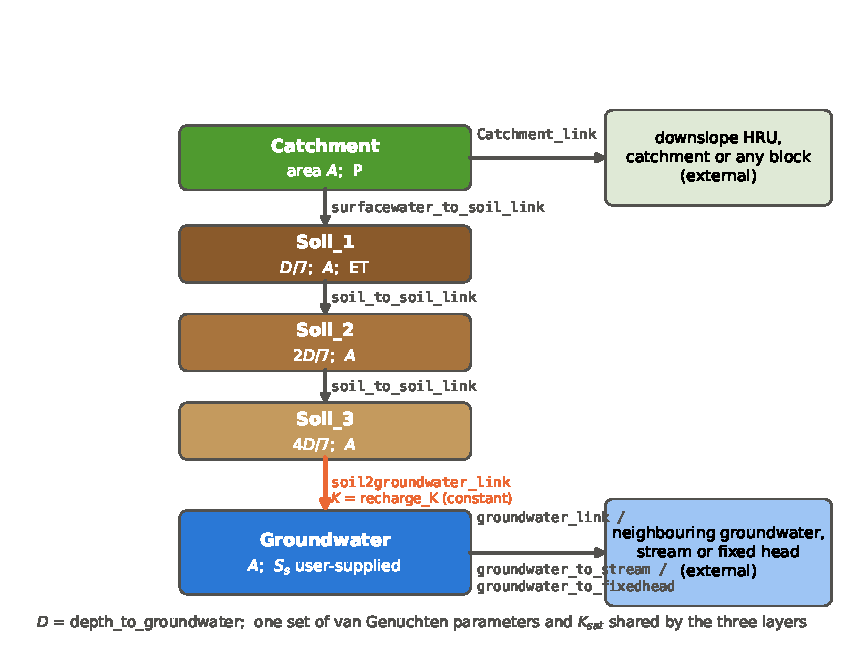
\includegraphics[width=0.8\textwidth]{hru_structure}
\caption{\code{Hydrologic\_Response\_Unit}: members, internal links and ports.}
\label{fig:hru}
\end{figure}

The HRU (\file{hydrologic\_response\_unit.json}, \cref{fig:hru}) has five members --- a
\code{Catchment} and the shared soil column and groundwater cell --- and four internal links. All of
them receive the whole plan area $A$. It has no internal reaches: the surface drains through its
\code{Catchment\_link} port directly to whatever block it is linked to, which makes cascades of units
possible (the overland flow of an upslope unit runs onto the surface of the next). Its ports:

\begin{table}[H]
\centering\small
\begin{tabular}{llp{6.1cm}c}
\toprule
Port (link type) & From member & Typical target & Icon \\
\midrule
\code{Catchment\_link} & \code{Catchment} & a downslope HRU, a catchment, a channel or any block & \raisebox{-0.4\height}{\includegraphics[height=0.9cm]{Catchment_outlet.png}} \\
\code{groundwater\_link} & \code{Groundwater} & the groundwater cell of a neighbouring unit & \raisebox{-0.4\height}{\includegraphics[height=0.9cm]{Groundwater_link.png}} \\
\code{groundwater\_to\_stream} & \code{Groundwater} & a channel segment (baseflow) & \raisebox{-0.4\height}{\includegraphics[height=0.9cm]{GW_to_Stream.png}} \\
\code{groundwater\_to\_fixedhead} & \code{Groundwater} & a \code{fixed\_head} block & \raisebox{-0.4\height}{\includegraphics[height=0.9cm]{gw_2_fixed_head.png}} \\
\bottomrule
\end{tabular}
\end{table}

\noindent Recharge uses the stock \code{soil2groundwater\_link} with the constant conductivity
\code{recharge\_K}, $Q_r=A\,K_{rech}(h_3-h_g)/L$ with $L=\tfrac12(d_3+b)$, and the groundwater cell's
head is $h_g=z_g+b+(\theta_g-\phi)/S_s$ with user-supplied $\phi$ and $S_s$. One set of soil parameters
applies to all three layers. The caveats of \cref{sec:mixedspec} about deep water tables and the
confined-style default $S_s$ apply to the HRU as well. A two-unit hillslope using it is in
\exfile{Examples/Hydrologic\_Response\_Unit/HRU\_hillslope.ohq}.

\section{Structure of the Urban (and Mixed) HRU}
\label{sec:common}

\Cref{fig:urban} shows the Urban HRU and \cref{fig:mixed} the legacy Mixed HRU, which has the same
members. Each has eight members:

\begin{itemize}[leftmargin=1.4em]
\item \code{Catchment} --- the pervious (infiltrating) surface;
\item \code{Impervious\_Catchment} --- the impervious surface, with no connection to any soil;
\item \code{Reach}, \code{Impervious\_Reach} --- two \code{Trapezoidal Channel Segment}s that collect
      the runoff of each surface: the swales, gutters, small streams and storm pipes inside the unit;
\item \code{Soil\_1}, \code{Soil\_2}, \code{Soil\_3} --- three van Genuchten soil layers under the
      pervious surface;
\item \code{Groundwater} --- a \code{Groundwater cell}.
\end{itemize}

\noindent and six internal links: a \code{Catchment\_link} from each surface to its reach,
infiltration (\code{surfacewater\_to\_soil\_link}) from the pervious surface into \code{Soil\_1},
percolation (\code{soil\_to\_soil\_link}) from \code{Soil\_1} to \code{Soil\_2} and from
\code{Soil\_2} to \code{Soil\_3}, and recharge from \code{Soil\_3} into the groundwater cell.



\begin{figure}[H]
\centering
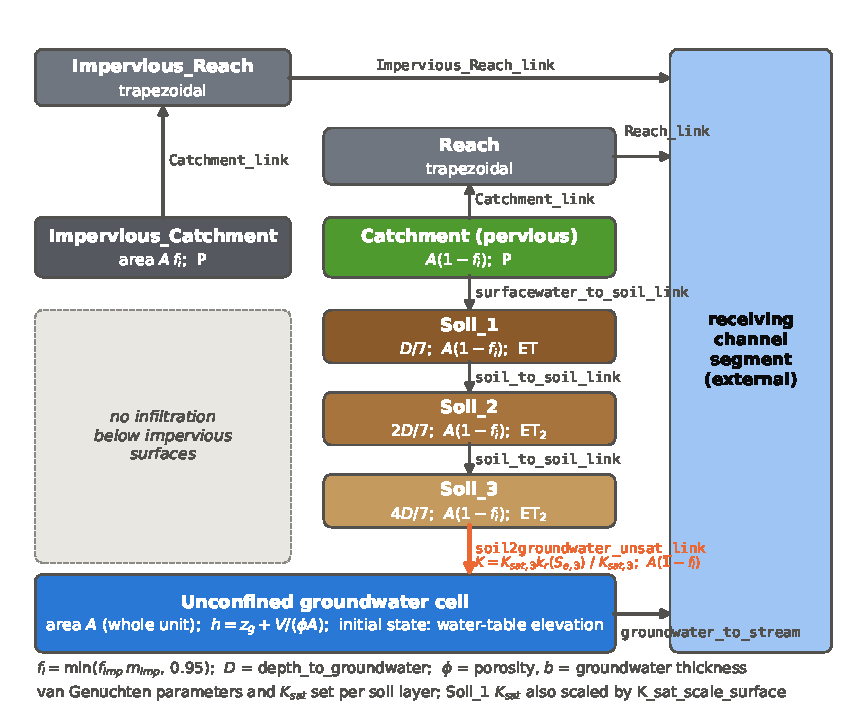
\includegraphics[width=0.86\textwidth]{urban_hru_structure}
\caption{\code{Urban\_HRU}: members (boxes, with thickness and plan area), internal links (arrows)
and ports to the receiving channel segment. The recharge connector is highlighted.}
\label{fig:urban}
\end{figure}

\begin{figure}[H]
\centering
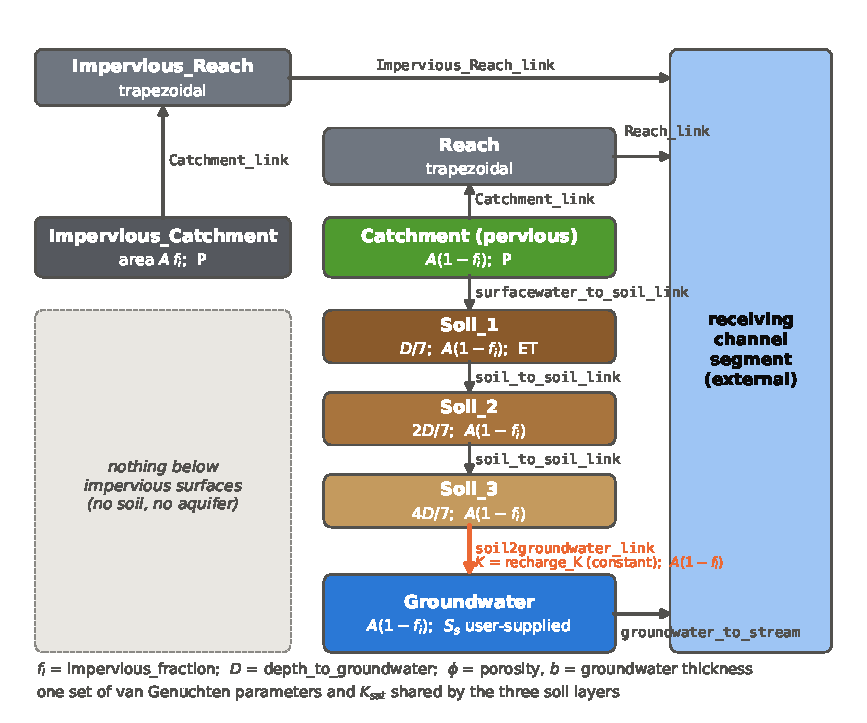
\includegraphics[width=0.86\textwidth]{mixed_hru_structure}
\caption{The legacy \code{Mixed\_Hydrologic\_Response\_Unit}. Differences from \cref{fig:urban}: the
groundwater cell has only the pervious area, recharge uses a constant conductivity, and the
groundwater specific storage is user-supplied.}
\label{fig:mixed}
\end{figure}

\subsection{Ports}
\label{sec:ports}
A composite exposes the members that may be connected from outside as \emph{ports}. Both units
declare the same five:

\begin{table}[H]
\centering\small
\begin{tabular}{llp{6.3cm}c}
\toprule
Port (link type) & From member & Typical target & Icon \\
\midrule
\code{Reach\_link} & \code{Reach} & the receiving channel segment & \raisebox{-0.4\height}{
\includegraphics[height=0.9cm]{HRU_Pervious_Outlet.png}} \\
\code{Impervious\_Reach\_link} & \code{Impervious\_Reach} & the receiving channel segment & \raisebox{-0.4\height}{
\includegraphics[height=0.9cm]{HRU_Impervious_Outlet.png}} \\
\code{groundwater\_to\_stream} & \code{Groundwater} & a channel segment (baseflow) & \raisebox{-0.4\height}{\includegraphics[height=0.9cm]{GW_to_Stream.png}} \\
\code{groundwater\_link} & \code{Groundwater} & the groundwater cell of a neighbouring unit & \raisebox{-0.4\height}{\includegraphics[height=0.9cm]{Groundwater_link.png}} \\
\code{groundwater\_to\_fixedhead} & \code{Groundwater} & a \code{fixed\_head} block & \raisebox{-0.4\height}{\includegraphics[height=0.9cm]{gw_2_fixed_head.png}} \\
\bottomrule
\end{tabular}
\end{table}

\code{Reach\_link} and \code{Impervious\_Reach\_link} are defined in
\file{mixed\_hydrologic\_response\_unit.json} and are used by both units. Their equations are those of
the channel-to-channel connector (\code{Trapezoidal\_Channel\_link}); they exist as separate types
only so that the two outlets of one composite can be told apart when a link is drawn from it, and
they have their own icons so that HRU outlets are distinguishable from links along the stream
network. When a link is drawn from an HRU in the interface, the port whose type matches the chosen
link is used; in a script, \code{create link;type=Reach\_link,from=SC01,to=R01} connects the
\code{Reach} member of \code{SC01}.

\subsection{Surface runoff and routing}
Rain falls on both surfaces. Water on a surface drains to its reach with the kinematic sheet-flow
relation of \code{Catchment\_link},
\begin{equation}
  Q_s = 86400\,\frac{W}{n_s}\,S^{1/2}\,\big(d-d_s\big)_+^{5/3},
\end{equation}
with overland width $W$ (\code{catchment\_width}), slope $S$ (\code{catchment\_slope}), Manning
coefficient $n_s$, ponded depth $d$ and depression storage $d_s$; $(x)_+=\max(x,0)$. Both surfaces
share $W$ and $S$ and have their own $n_s$ and $d_s$. The reaches drain to the receiving segment
through the outlet ports with Manning's equation driven by the head difference,
\begin{equation}
  Q_r = 86400\,\frac{1}{\bar n}\,A_u\,R^{2/3}\left(\frac{h_r-h_c}{\bar L}\right)^{1/2},
  \qquad \bar L=\tfrac12\,(L_r+L_c),\quad \bar n=\tfrac12\,(n_r+n_c),
  \label{eq:outlet}
\end{equation}
where $A_u$ is the flow area of the end with the higher head, $R$ the hydraulic radius from the
mean perimeter, and subscripts $r$ and $c$ refer to the internal reach and the receiving channel.
The reach bottoms are placed at the surface elevation.

\subsection{The impervious fraction}
\label{sec:impfrac}
The impervious surface drains directly to the internal impervious reach and from there to the
channel, with no chance to infiltrate. \code{impervious\_fraction} must therefore be the
\emph{directly connected} impervious area (DCIA) --- roofs, roads and parking areas whose runoff
reaches a storm drain or the stream without crossing pervious ground --- and not the total impervious
area (TIA) mapped from land cover. The composites take it as a plain number; how it is estimated is
up to the modeller. Common choices:

\begin{itemize}[leftmargin=1.4em]
\item \textbf{Empirical TIA--DCIA relations.} Sutherland (2000) gives DCIA as a function of TIA (both
  in percent, for TIA\,$\ge$\,1\,\%) for five degrees of connectivity:
  \begin{center}\small
  \begin{tabular}{ll}
  \toprule
  Drainage & DCIA \\
  \midrule
  Totally connected (curb, gutter and storm sewer; roofs tied in) & TIA \\
  Highly connected & $0.4\,\mathrm{TIA}^{1.2}$ \\
  Average (mostly storm-sewered, some roofs to lawns) & $0.1\,\mathrm{TIA}^{1.5}$ \\
  Somewhat disconnected & $0.04\,\mathrm{TIA}^{1.7}$ \\
  Highly disconnected (swales, roofs to lawns) & $0.01\,\mathrm{TIA}^{2}$ \\
  \bottomrule
  \end{tabular}
  \end{center}
\item \textbf{Storm-drain inventories.} Where inlet locations are available, impervious surfaces
  within a set distance of an inlet (or of a guttered street that leads to one) can be counted as
  connected. Public inventories miss private systems, so this tends to be a lower bound.
\item \textbf{Calibration.} In the Urban HRU the estimate is scaled by
  \code{impervious\_multiplier} (\cref{sec:multipliers}); keeping each unit's estimate and
  calibrating one multiplier preserves the spatial pattern and adjusts the level.
\end{itemize}

\noindent Impervious surfaces that are \emph{not} directly connected remain part of the pervious
surface (\cref{sec:disconnected}).

%==========================================================================================
\section{Mixed HRU (legacy)}
\label{sec:mixedspec}

The Mixed HRU (\file{mixed\_hydrologic\_response\_unit.json}) is not listed in the interface. It
remains in the repository so that models built with it open and run unchanged, and because the
\code{Reach\_link} and \code{Impervious\_Reach\_link} types used by the Urban HRU are defined in its file.
It differs from the Urban HRU in six ways (\cref{sec:differences}), so the Urban HRU does not reproduce
it; results change when a model is moved from one to the other.

\paragraph{Areas.} With $f_i$ = \code{impervious\_fraction} (strictly between 0 and 1):
$A f_i$ for \code{Impervious\_Catchment}; $A(1-f_i)$ for \code{Catchment}, the three soil layers,
the recharge interface \emph{and} the groundwater cell. Nothing lies below the impervious surface.

\paragraph{Soil.} One set of $K_{sat}$, $\alpha$, $n$, $\theta_s$, $\theta_r$ applies to all three
layers, which then discretise a single profile.

\paragraph{Recharge.} \code{soil2groundwater\_link}:
\begin{equation}
  Q_r = A(1-f_i)\,K_{rech}\,\frac{h_3-h_g}{L},\qquad L=\tfrac12\,(d_3+b),
\end{equation}
with the constant \code{recharge\_K}.

\paragraph{Groundwater.} $h_g=z_g+b+(\theta_g-\phi)/S_s$ with user-supplied porosity $\phi$ and specific
storage $S_s$. With the defaults ($S_s=0.01$\,m$^{-1}$, $\theta_{g,0}=\phi=0.4$) the cell starts full
and responds as a \emph{confined} aquifer: a change of 0.01 in moisture content moves the head by
1\,m.

%==========================================================================================
\section{Urban HRU}
\label{sec:urbanspec}

\subsection{Areas}
With $f_i=\min(f_{imp}\,m_{imp},\,0.95)$, where $f_{imp}$ is \code{impervious\_fraction} and $m_{imp}$
the \code{impervious\_multiplier}:

\begin{table}[H]
\centering\small
\begin{tabular}{ll}
\toprule
Member & Plan area \\
\midrule
\code{Impervious\_Catchment} & $A\,f_i$ \\
\code{Catchment}, \code{Soil\_1}--\code{Soil\_3}, recharge interface & $A\,(1-f_i)$ \\
\code{Groundwater} & $A$ \\
\bottomrule
\end{tabular}
\end{table}

\noindent The aquifer continues beneath roads and roofs, so the groundwater cell receives the whole
area; it is recharged only through the pervious soil column. With the pervious area instead (as in the
Mixed HRU) the water table would rise $1/(1-f_i)$ times too fast per unit of recharge --- twice as fast
at $f_i=0.5$ --- and any change of $f_i$ during calibration would also change the aquifer.

\subsection{Recharge through the unsaturated conductivity}
\label{sec:recharge}
\code{soil2groundwater\_unsat\_link} (\file{groundwater.json}) connects \code{Soil\_3} (the source,
which must be a \code{Soil} block) to the groundwater cell:
\begin{equation}
  Q_r = A(1-f_i)\,K_{sat,3}\;
        \frac{k_r(S_{e,3})\,\big(h_3-h_g\big)_+ \;-\; \big(h_g-h_3\big)_+}{L},
        \qquad L=\tfrac12\,(d_3+b).
  \label{eq:recharge}
\end{equation}
When the soil head is higher (drainage) the conductivity is the unsaturated conductivity of the bottom
layer, with the same Mualem $k_r$ as the percolation links; when the groundwater head is higher
(upward flow) the saturated conductivity is used.

The reason is the depth of urban and upland water tables. When the water table lies several metres or
more below the soil column, $h_3-h_g$ is dominated by elevation and hardly depends on how wet the soil
is. With a constant conductivity the flux is then almost independent of soil moisture: in a
watershed application with the water table 6--47\,m below the soil and $K_{rech}=0.1$\,m/d, the
constant-$K$ link gave a potential recharge of about 150\,mm/d at $S_e=0.5$, and at $S_e=0.2$ the
suction of the bottom layer reversed it into up to 380\,mm/d of upward flow from the deep water
table. Calibrating $K_{rech}$ can only trade one error for the other. With \eqref{eq:recharge} the
flux falls with $k_r$ as the bottom layer drains, and no separate recharge conductivity is needed.

\subsection{Unconfined groundwater}
The composite sets the cell's specific storage to $S_s=\phi/b$ (\code{groundwater\_porosity} over
\code{groundwater\_thickness}), so that
\begin{equation}
  h_g = z_g + b\,\frac{\theta_g}{\phi}:
\end{equation}
the water table rises by $1/\phi$ per unit depth of stored water, as in an unconfined aquifer with
specific yield $\phi$. Because $S_s$ is computed inside the composite, this stays true when $\phi$ is
calibrated. To start with the water table at elevation $h_0$, set
\code{initial\_groundwater\_moisture\_content} to $\theta_{g,0}=\phi\,(h_0-z_g)/b$.

\subsection{Layer-specific soil}
\code{K\_sat\_}$i$, \code{alpha\_vG\_}$i$, \code{n\_vG\_}$i$, \code{theta\_sat\_}$i$ and
\code{theta\_res\_}$i$ ($i=1,2,3$) are set for each layer, for example from soil-survey horizons
averaged over the three depth intervals. The \code{K\_sat\_}$i$ go to each layer's
\code{K\_sat\_original}, so that the layer's \code{K\_sat\_scale\_factor} remains free for the
multiplier below.

\subsection{Calibration multipliers}
\label{sec:multipliers}
Both default to 1 and leave the unit unchanged at that value.

\begin{description}[leftmargin=1.4em,style=nextline]
\item[\code{impervious\_multiplier} ($m_{imp}$)] scales the impervious fraction:
  $f_i=\min(f_{imp}\,m_{imp},0.95)$. It is meant for calibrating the \emph{directly connected}
  impervious area watershed-wide when $f_{imp}$ comes from an empirical estimate. $m_{imp}>1$ means
  that more of the land drains straight to the channel than the estimate says (for example, more
  roofs and driveways tied to the storm drains); $m_{imp}<1$ means more of the impervious surface is
  disconnected. Area moves between the impervious catchment and the pervious catchment with its soil
  column; the total stays $A$ and the groundwater cell is unaffected. Infiltration, soil storage,
  \code{Soil\_1} evapotranspiration and recharge scale with the pervious area; the internal reaches and
  the \code{groundwater\_to\_stream} link do not change. $f_{imp}$ itself (for example a Sutherland
  estimate, \cref{sec:impfrac}) is fixed when the model is built; only $m_{imp}$ is calibrated.
\item[\code{K\_sat\_scale}] multiplies $K_{sat}$ of all three layers, and therefore also the
  recharge conductivity of \eqref{eq:recharge}.
\end{description}

\noindent Bind a model parameter to them at the composite level,
\begin{lstlisting}[style=plain]
create parameter;type=Parameter,name=p_imp,low=0.3,high=3,value=1,prior_distribution=log-normal
setasparameter; object=SC01, quantity=impervious_multiplier, parametername=p_imp
\end{lstlisting}
and the value reaches the members through the composite's mappings. When a parameter changes, the
member areas are re-evaluated and the initial soil storages $\theta_0A_\ell d_\ell$ recomputed, so the
initial moisture content stays $\theta_0$; the code generator (\code{ohq\_generate}) compiles the same
mappings and initial storages as expressions of the parameter vector.

\subsection{Disconnected impervious area}
\label{sec:disconnected}
Only the \emph{connected} impervious fraction is an impervious surface. Impervious surfaces that drain
onto lawns --- roofs with leaders to splash blocks, driveways sloping to grass --- belong to the
pervious catchment $A(1-f_i)$ and are treated as soil: rain on them can infiltrate, and the
\code{Soil\_1} evapotranspiration and the recharge interface act over them. Neither the concentration
of their runoff onto the adjacent lawn nor the absence of transpiration from roofs is represented. If
that matters, a third \code{Catchment} for the disconnected area, joined to \code{Catchment} by a
\code{Catchment\_link}, would represent both; it is not part of the composite.

%==========================================================================================
\section{Urban HRU versus Mixed HRU}
\label{sec:differences}
The two units share their members, surface routing and ports; the subsurface and the parameters
differ:

\begin{table}[H]
\centering\small
\begin{tabular}{p{3.6cm}p{5.4cm}p{5.4cm}}
\toprule
 & Mixed HRU & Urban HRU \\
\midrule
Groundwater area & $A(1-f_i)$ & $A$ \\
Recharge link & \code{soil2groundwater\_link}, constant \code{recharge\_K} & \code{soil2groundwater\_unsat\_link}, $K_{sat,3}k_r(S_{e,3})$ / $K_{sat,3}$ \\
Groundwater storage & user $S_s$ (default: confined) & $S_s=\phi/b$ (unconfined) \\
Soil parameters & \code{K\_sat}, \code{alpha\_vG}, \code{n\_vG}, \code{theta\_sat}, \code{theta\_res} & the same with suffix \code{\_1}, \code{\_2}, \code{\_3} \\
Properties only here & \code{recharge\_K}, \code{groundwater\_specific\_storage} & \code{impervious\_multiplier}, \code{K\_sat\_scale} \\
Impervious fraction & $0<f_i<1$ & $f_i=\min(f_{imp}m_{imp},0.95)$ \\
Default \code{groundwater\_porosity} / initial moisture & 0.4 / 0.4 (full cell) & 0.2 / 0.1 (half full) \\
In the template list & no & yes \\
\bottomrule
\end{tabular}
\end{table}

%==========================================================================================
\section{Using the units}

\subsection{Templates}
The HRU lists \file{main\_components.json}, \file{unsaturated\_soil.json} and \file{groundwater.json} in
its \code{requires}. The Urban HRU lists \file{main\_components.json}, \file{unsaturated\_soil.json},
\file{groundwater.json}, \file{open\_channel.json} and \file{mixed\_hydrologic\_response\_unit.json}
(for the outlet ports) in its \code{requires}, so selecting it alone in the interface is enough. The
evapotranspiration source is not a member; load \file{soil\_evapotranspiration\_models.json} for the
\code{Evapotranspiration\_Time\_Series (Soil)} source.

\subsection{A minimal model}
\exdir{Examples/Mixed\_Urban\_HRU} holds two models with identical inputs: one 50\,ha unit with 25\,\%
impervious area, draining to an 800\,m trapezoidal stream that ends at a fixed head, forced by 30 days
of hourly rain and daily reference ET. The Urban HRU version:

\begin{lstlisting}[style=plain]
loadtemplate; filename = main_components.json
addtemplate; filename = unsaturated_soil.json
addtemplate; filename = groundwater.json
addtemplate; filename = open_channel.json
addtemplate; filename = soil_evapotranspiration_models.json
addtemplate; filename = mixed_hydrologic_response_unit.json
addtemplate; filename = urban_hru.json
create source;type=Precipitation,name=Rain,timeseries=precipitation.csv
create source;type=Evapotranspiration_Time_Series (Soil),name=ET,corr_fact=0.8,ET_timeseries=evapotranspiration.csv
create composite;type=Urban_HRU,name=Neighbourhood,area=500000,impervious_fraction=0.25,
    surface_elevation=100,depth_to_groundwater=3.5,groundwater_thickness=12,
    Precipitation=Rain,Evapotranspiration=ET,catchment_slope=0.03,catchment_width=2500,
    K_sat_1=0.6,K_sat_2=0.4,K_sat_3=0.8,alpha_vG_1=1.5,...,
    groundwater_porosity=0.15,initial_groundwater_moisture_content=0.05,
    reach_length=400,impervious_reach_length=400,...
create block;type=Trapezoidal Channel Segment,name=Stream,base_width=3,side_slope=2,
    ManningCoeff=0.035,bottom_elevation=88,length=800,depth=0.1
create block;type=fixed_head,name=Outlet,head=87
create link;type=Reach_link,from=Neighbourhood,to=Stream,name=Pervious_outlet
create link;type=Impervious_Reach_link,from=Neighbourhood,to=Stream,name=Impervious_outlet
create link;type=groundwater_to_stream,from=Neighbourhood,to=Stream,name=Baseflow,
    area=8000,length=150,hydraulic_conductivity=5
create link;type=channel2fixed,from=Stream,to=Outlet,name=Stream_outlet
\end{lstlisting}

\noindent(Line breaks inside \code{create} commands are for display only.) The Mixed HRU version
replaces the layer-specific soil parameters with the first layer's values and sets
\code{recharge\_K}\,=\,0.1\,m/d and \code{groundwater\_specific\_storage}\,=\,$\phi/b$ = 0.0125\,m$^{-1}$,
so that both start from the same water table. Members are addressed as
\code{Neighbourhood\_\_Soil\_3}, \code{Neighbourhood\_\_recharge} and so on in outputs and scripts.

\subsection{What the example shows}
\Cref{fig:example} and \cref{tab:example} compare the two runs. The surfaces behave identically:
all impervious runoff reaches the stream, and the pervious surface produces almost none because the
rain rate rarely exceeds the infiltration capacity. The difference is in the subsurface. With the
constant recharge conductivity the Mixed HRU passes more water to the aquifer in 30 days than
infiltrates, because it also drains the initial storage of the soil column (recharge of 90\,mm/d on
the first day, independent of soil moisture), and the smaller groundwater area amplifies the rise of
the water table. The Urban HRU's recharge follows the unsaturated conductivity, starts at 8\,mm/d
and settles near the rate at which water percolates through the column.

\begin{figure}[H]
\centering
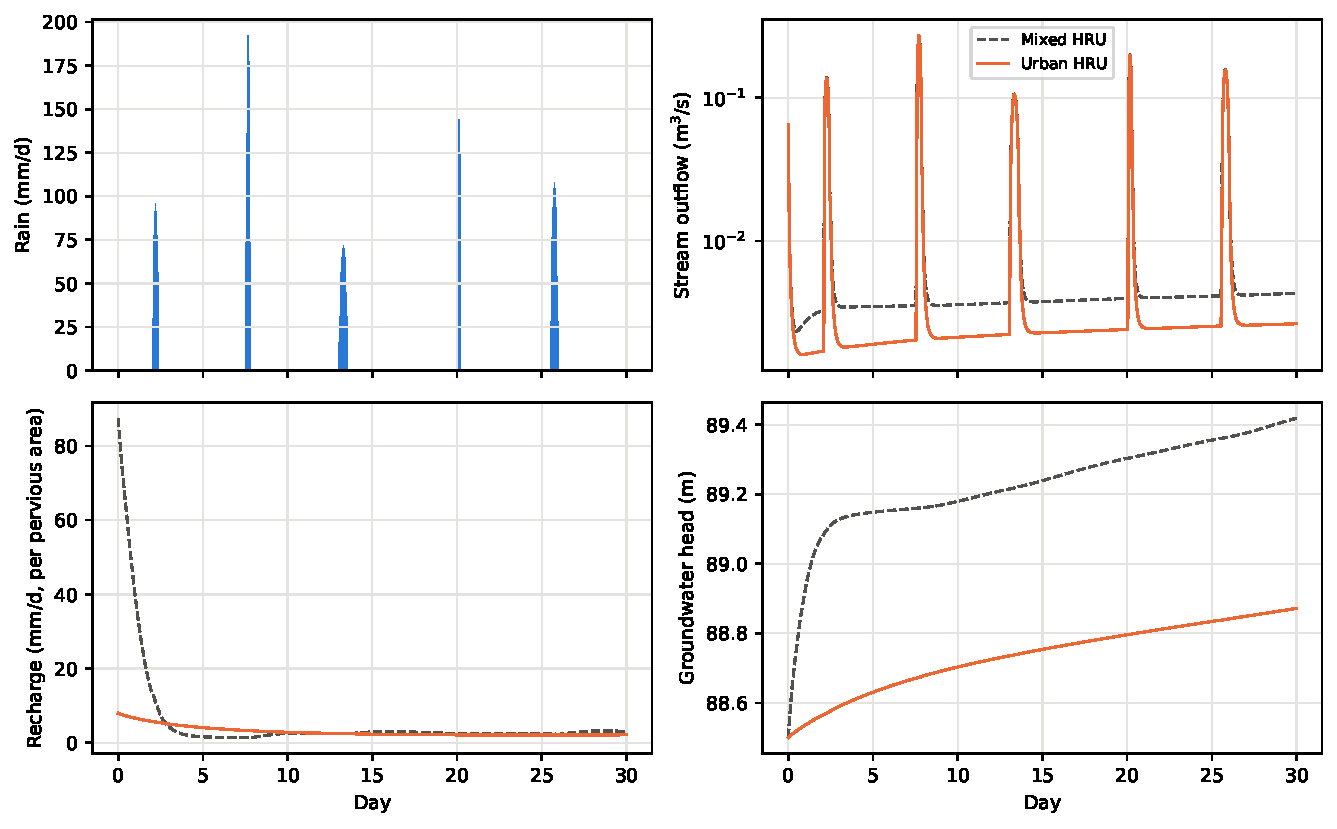
\includegraphics[width=\textwidth]{hru_example_comparison}
\caption{Mixed and Urban HRU with identical inputs (\exdir{Examples/Mixed\_Urban\_HRU}).}
\label{fig:example}
\end{figure}

\begin{table}[H]
\centering\small
\begin{tabular}{lrr}
\toprule
Volume over 30 days (m$^3$) & Mixed HRU & Urban HRU \\
\midrule
Rain & 74,336 & 74,336 \\
Impervious outlet (\code{Impervious\_Reach\_link}) & 18,363 & 18,370 \\
Pervious outlet (\code{Reach\_link}) & 4 & 4 \\
Infiltration & 55,750 & 55,749 \\
Recharge & 60,646 & 33,526 \\
Baseflow (\code{groundwater\_to\_stream}) & 9,645 & 5,717 \\
Stream outflow & 28,069 & 24,179 \\
\midrule
Groundwater head rise (m) & 0.92 & 0.37 \\
\bottomrule
\end{tabular}

\caption{Water balance of the two example runs.}
\label{tab:example}
\end{table}

%==========================================================================================
\section{Property reference}
\label{sec:reference}
Generated from the three resource files by \exfile{docs/make\_hru\_figures.py}. ``In'' gives the
units that expose the property (HRU, Mixed, Urban); ``Applied to'' lists the members that receive it;
where the defaults differ between units they are separated by a slash.

{\small
\begin{longtable}{p{4.9cm}p{1.3cm}p{1.2cm}p{1.9cm}p{4.7cm}}
\toprule
Property & Unit & Default & In & Applied to \\
\midrule
\endhead
\code{area} & m$^2$ & 1000 & all & member areas \\
\code{recharge\_K} & m/day & 1 & HRU, Mixed & recharge \\
\code{surface\_elevation} & m & 0 & all & Catchment, Groundwater, Impervious\_Catchment, Impervious\_Reach, Reach, Soil\_1, Soil\_2, Soil\_3 \\
\code{depth\_to\_groundwater} & m & 3.5 & all & Soil\_1, Soil\_2, Soil\_3 \\
\code{groundwater\_thickness} & m & 5 & all & Groundwater \\
\code{Precipitation} &  &  & all & Catchment, Impervious\_Catchment \\
\code{Evapotranspiration} &  &  & all & Soil\_1 \\
\code{catchment\_slope} &  & 0.01 & all & Catchment, Impervious\_Catchment \\
\code{catchment\_width} & m & 30 & all & Catchment, Impervious\_Catchment \\
\code{manning\_coefficient} &  & 0.05 & all & Catchment \\
\code{depression\_storage} & m & 0 & all & Catchment \\
\code{runoff\_coefficient} &  & 1 & all & Catchment, Impervious\_Catchment \\
\code{K\_sat} & m/day & 1 & HRU, Mixed & Soil\_1, Soil\_2, Soil\_3 \\
\code{alpha\_vG} & 1/m & 1 & HRU, Mixed & Soil\_1, Soil\_2, Soil\_3 \\
\code{n\_vG} &  & 1.41 & HRU, Mixed & Soil\_1, Soil\_2, Soil\_3 \\
\code{theta\_sat} &  & 0.4 & HRU, Mixed & Soil\_1, Soil\_2, Soil\_3 \\
\code{theta\_res} &  & 0.05 & HRU, Mixed & Soil\_1, Soil\_2, Soil\_3 \\
\code{soil\_specific\_storage} & 1/m & 0.01 & all & Soil\_1, Soil\_2, Soil\_3 \\
\code{initial\_moisture\_content} &  & 0.2 & all & Soil\_1, Soil\_2, Soil\_3 \\
\code{groundwater\_K} & m/day & 1 & all & Groundwater \\
\code{groundwater\_porosity} &  & 0.2/0.4 & all & Groundwater \\
\code{groundwater\_specific\_storage} & 1/m & 0.01 & HRU, Mixed & Groundwater \\
\code{initial\_groundwater\_moisture\_content} &  & 0.1/0.25/0.4 & all & Groundwater \\
\code{impervious\_fraction} &  & 0.2 & Mixed, Urban & member areas \\
\code{impervious\_manning\_coefficient} &  & 0.015 & Mixed, Urban & Impervious\_Catchment \\
\code{impervious\_depression\_storage} & m & 0.001 & Mixed, Urban & Impervious\_Catchment \\
\code{reach\_base\_width} & m & 1 & Mixed, Urban & Reach \\
\code{reach\_side\_slope} &  & 2 & Mixed, Urban & Reach \\
\code{reach\_manning\_coefficient} &  & 0.035 & Mixed, Urban & Reach \\
\code{reach\_length} & m & 10 & Mixed, Urban & Reach \\
\code{initial\_reach\_depth} & m & 0.01 & Mixed, Urban & Reach \\
\code{impervious\_reach\_base\_width} & m & 1 & Mixed, Urban & Impervious\_Reach \\
\code{impervious\_reach\_side\_slope} &  & 2 & Mixed, Urban & Impervious\_Reach \\
\code{impervious\_reach\_manning\_coefficient} &  & 0.02 & Mixed, Urban & Impervious\_Reach \\
\code{impervious\_reach\_length} & m & 10 & Mixed, Urban & Impervious\_Reach \\
\code{initial\_impervious\_reach\_depth} & m & 0.01 & Mixed, Urban & Impervious\_Reach \\
\code{K\_sat\_1} & m/day & 1 & Urban & Soil\_1 \\
\code{K\_sat\_2} & m/day & 1 & Urban & Soil\_2 \\
\code{K\_sat\_3} & m/day & 1 & Urban & Soil\_3 \\
\code{alpha\_vG\_1} & 1/m & 1 & Urban & Soil\_1 \\
\code{alpha\_vG\_2} & 1/m & 1 & Urban & Soil\_2 \\
\code{alpha\_vG\_3} & 1/m & 1 & Urban & Soil\_3 \\
\code{n\_vG\_1} &  & 1.41 & Urban & Soil\_1 \\
\code{n\_vG\_2} &  & 1.41 & Urban & Soil\_2 \\
\code{n\_vG\_3} &  & 1.41 & Urban & Soil\_3 \\
\code{theta\_sat\_1} &  & 0.4 & Urban & Soil\_1 \\
\code{theta\_sat\_2} &  & 0.4 & Urban & Soil\_2 \\
\code{theta\_sat\_3} &  & 0.4 & Urban & Soil\_3 \\
\code{theta\_res\_1} &  & 0.05 & Urban & Soil\_1 \\
\code{theta\_res\_2} &  & 0.05 & Urban & Soil\_2 \\
\code{theta\_res\_3} &  & 0.05 & Urban & Soil\_3 \\
\code{impervious\_multiplier} &  & 1 & Urban & member areas \\
\code{K\_sat\_scale} &  & 1 & Urban & Soil\_1, Soil\_2, Soil\_3 \\
\bottomrule
\end{longtable}

}

%==========================================================================================
\section{Limitations and pitfalls}
\begin{itemize}[leftmargin=1.4em]
\item \textbf{Fixed layer split.} The three soil layers are always $D/7$, $2D/7$ and $4D/7$; $D$
  controls the storage, the recharge path length and the heads together, so calibrating it moves all
  three at once.
\item \textbf{Deep water tables.} When the water table is far below the soil column, the Mixed HRU's
  constant recharge conductivity drains the column regardless of its wetness and pulls water upward
  when the bottom layer dries (\cref{sec:recharge}); use the Urban HRU or keep \code{recharge\_K}
  small.
\item \textbf{Confined-style defaults in the Mixed HRU.} With $S_s=0.01$\,m$^{-1}$ the head responds
  metres to small changes of storage. For an unconfined aquifer set $S_s=\phi/b$.
\item \textbf{Outlet link length.} \eqref{eq:outlet} averages the length of the internal reach with
  that of the receiving segment, so a long receiving segment lowers the outlet slope.
\item \textbf{Internal reaches are generic.} Their shape and roughness are properties of the unit,
  not derived from its drainage network; they mostly control the timing of the runoff peak.
\item \textbf{Evapotranspiration from \code{Soil\_1} only.} Deeper layers and the groundwater cell do
  not transpire; the rate is scaled by $\theta/\theta_s$ of the top layer.
\item \textbf{Disconnected impervious area} is treated as pervious soil (\cref{sec:urbanspec}).
\item \textbf{One unit, one soil column.} Spatial variation inside a sub-catchment is represented
  only through its areas; use more units for more variation.
\end{itemize}

\section*{Reference}
\noindent Sutherland, R.\,C. (2000). Methods for estimating the effective impervious area of urban
watersheds. \emph{Watershed Protection Techniques} 2(4), 282--284.

\end{document}
